\documentclass[a4paper,twoside,11pt, fleqn]{article}
\usepackage{a4wide,graphicx,fancyhdr,amsmath,amssymb}
\usepackage{listings}
\usepackage{color}
\usepackage{dirtree}
\usepackage{subcaption}

%matlab 
\usepackage[]{mcode}

%----------------------- Macros and Definitions --------------------------

\setlength\headheight{20pt}
\addtolength\topmargin{-10pt}
\addtolength\footskip{20pt}

\newcommand{\N}{\mathbb{N}}
\newcommand{\ch}{\mathcal{CH}}

\newcommand{\solution}[1]{\noindent{\bf Solution to Exercise #1:}}

\fancypagestyle{plain}{%
\fancyhf{}
\fancyhead[LO,RE]{\sffamily\bfseries\large technische universiteit eindhoven}
\fancyhead[RO,LE]{\sffamily\bfseries\large 2IN35 VLSI}
\fancyfoot[LO,RE]{\sffamily\bfseries\large department of mathematics and computer science}
\fancyfoot[RO,LE]{\sffamily\bfseries\thepage}
\renewcommand{\headrulewidth}{0pt}
\renewcommand{\footrulewidth}{0pt}
}

\pagestyle{fancy}
\fancyhf{}
\fancyhead[RO,LE]{\sffamily\bfseries\large technische universiteit eindhoven}
\fancyhead[LO,RE]{\sffamily\bfseries\large 2IN35 VLSI}
\fancyfoot[LO,RE]{\sffamily\bfseries\large department of mathematics and computer science}
\fancyfoot[RO,LE]{\sffamily\bfseries\thepage}
\renewcommand{\headrulewidth}{1pt}
\renewcommand{\footrulewidth}{0pt}

\def\addsquare#1{\tikz\node[draw]{#1};} 

%-------------------------------- Title ----------------------------------

\title{\vspace{-\baselineskip}\sffamily\bfseries Assignment 4}
\author{
	Rick Veens \qquad Studentno: 0912292\\
	\texttt{r.veens@student.tue.nl}
	\and
	Barry de Bruin \qquad Studentno: 0919605\\
	\texttt{e.d.bruin@student.tue.nl}
	\and
	\texttt{Group 7}
}

\date{\today}

\setlength\parindent{0pt}

%--------------------------------- Text ----------------------------------

\begin{document}
\maketitle
\newpage

\tableofcontents

\newpage

\section{Exercise 1}
Figure \ref{fig:flow} describes the general flow of an resampler. We are going to verify the direct equation solution.
\begin{figure}[h]
	\centering
	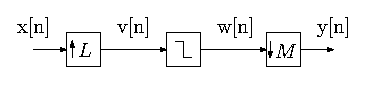
\includegraphics[scale = 1.3]{Images/3_01}
    \caption{resampler flow}
    \label{fig:flow}
\end{figure}

We can define the filter equation as a convolution sum:
\begin{align*}
w[n] 	&= \sum_{0\leq k < 4L} h[k]\cdot v[n-k]\text{, for k $\in \mathbb{N}$}\\
\intertext{Unroll the summation sign by defining k = jL + l, where j,l  $\in \mathbb{N}$}
		&= \sum_{0\leq j<4}  \sum_{0\leq l<L} h[jL + l]\cdot v[n-(jL+l)]		
\end{align*}
We want to end with a function where x is the input, and y is the output. Therefore we are going to express both x and y in v and w and try to substitute them in the convolution sum.

\begin{figure}[h]
	\centering
	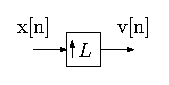
\includegraphics[scale = 1.3]{Images/3_02}
    \caption{Upsampling part}
     \label{fig:up}
\end{figure}

Upsampling the input sample means that for every input sample we will have $L$ output samples. Therefore we can define the part of figure \ref{fig:up} as:\\

$ v[n] =
  \begin{cases}
    x[\dfrac{n}{L}]      & \quad \text{if } n \text{\textbf{ mod }} L = 0\\
    0  					& \quad \text{if } n \text{\textbf{ mod }} L \neq 0\\
  \end{cases}$

\begin{figure}[h]
	\centering
	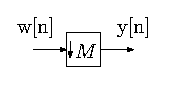
\includegraphics[scale = 1.3]{Images/3_03}
    \caption{Downsampling part}
    \label{fig:down}
\end{figure}

For the downsampling part that is shown in figure \ref{fig:down}, we can say that for every M inputs, we want one output, or:\\

$y[n] = w[n\cdot m]$\\

Substituting x and y in the convolution sum yields:\\

$ v[n - (jL + l)] =
  \begin{cases}
    x[\dfrac{n - (jL + l)}{L}]      & \quad \text{if } n - (jL + l) \text{\textbf{ mod }} L = 0\\
    0  					& \quad \text{if } n - (jL + l) \text{\textbf{ mod }} L \neq 0\\
  \end{cases}$
  
Therefore we can substitute this into our function:\\

$w[n] = \sum_{0\leq j<4}  \sum_{0\leq l<L} h[jL + l]\cdot x[\dfrac{n - (jL + l)}{L}]$ , for $n - (jL + l) \textbf{ mod } L = 0$\\

now rewrite:
\begin{align*}
n - (jL + l) \textbf{ mod } L = 0\\
n - jL - l \textbf{ mod } L = 0\\
n - jL \textbf{ mod } L = l\\
\end{align*}
Substitute in for this in function w(n):
\begin{align*}
w[n] &= \sum_{0\leq j<4}  \sum_{0\leq l<L} h[jL + n - jL \textbf{ mod } L]\cdot x[\dfrac{n - jL + (n - jL) \textbf{ mod } L}{L}]\\
	 &= \sum_{0\leq j<4}  \sum_{0\leq l<L} h[jL + (n - jL \textbf{ mod } L]\cdot x[\dfrac{n}{L} - {j}  - \dfrac{(n - jL \textbf{ mod } L))}{L}]\\
\end{align*}

\textbf{Don't know how to get rid of the factor in x, the last step should be to substitute y for w.}


\newpage
\section{Exercise 2}
If we take for example L = 5 and M = 4, we get the following results:
\begin{figure}[h]
	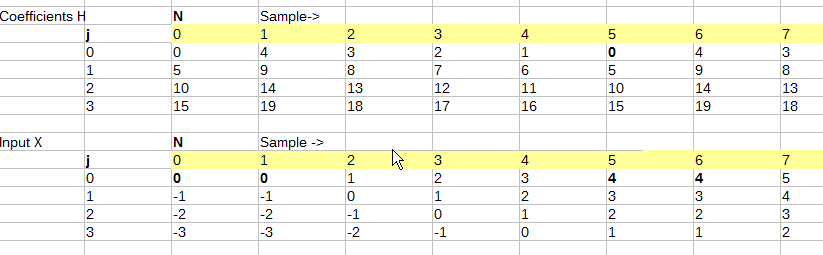
\includegraphics[scale = 0.8]{Images/repeat}
    \caption{Direct equation input and coefficient plot for L = 5 and M = 4}
\end{figure}

One noteworthy aspect of the figure is that the first sample always get used twice, but with a different coefficient. The cycle will repeat after 5 cycles for both the coefficients and the input samples.

\section{Exercise 3}
We have the following 4 designs: 

\subsection{Direct equation solution}
This solution uses the direct equation and has two different implementations: The direct method that has a single direct equation stage, and the composite implementation that uses two stages.\\

\textbf{Direct method}\\
This implementation uses $4\cdot L$ coefficients and needs only 4 multiplications/additions. All inner factors can be pre-computed.
\smallskip
The highest sample rate inside the system (system frequency) will be input or output sample frequency, depending on the L and M constants. Therefore: $F_{system} = max(Fs_{in}, Fs_{out})$.]\\
 
\textbf{Composite method}\\
Uses $4\cdot (L_{sub1} + L_{sub2})$ coefficients, while $L = L_{sub1} \cdot L_{sub2}$. Therefore we need less coefficients compared to the direct method. Since every sample still needs 4 multiplications/additions, we actually need 8 multiplication/additions for this implementation.

\smallskip
If we compose a resampler of two of those systems, the highest system frequency will be input frequency of the first system, the output of the first system (input of second system), or the output of the second system.

\subsection{Naive solution}
Uses the complete part of an upscaler, low-pass filter and downscaler. Again we have two variants:\\

\textbf{Direct scalers}\\
Since the filter in this implementation is just a low-pass FIR filter, we need one multiplication/addition step for every coefficient. This is not very efficient because L-1 out of L samples are zero and will therefore not influence the output signal. Because $4\cdot L$ coefficients are needed to filter out the high-frequency noise, we need the same amount of multiplication/additions for one output sample.

\smallskip
The maximum system frequency will be $F_{system} = F_s\cdot L$ Hz, which is the sampling frequency of the low-pass filter. This is also shown in figure \ref{fig:naive} below:
\begin{figure}[h]
	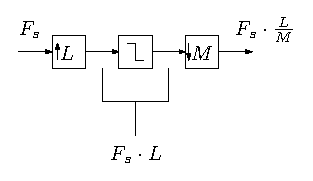
\includegraphics[scale = 1]{Images/3_0}
    \caption{Naive solution with single set of stages}
    \label{fig:naive}
\end{figure}

\textbf{Composite scalers } \\
Now we actually have two stages and therefore we need to apply the FIR filter in both stages. This will actually cost us $4\cdot (L_1 + L_2)$ multiplication/addition steps, where still L-1 out of L samples are zero.

\smallskip
The maximum system frequency will be $F_{system} = max(F_s\cdot L_1, F_s\cdot \frac{L_1\cdot L_2}{M_1})$, since one of the two stages can have the highest frequency, depending on the L and M parameters.
\begin{figure}[h]
	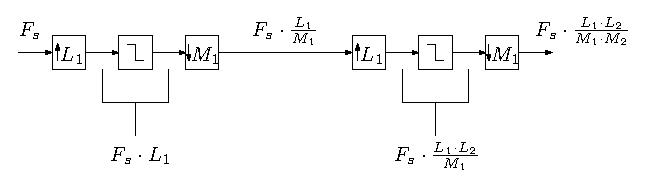
\includegraphics[scale = 1]{Images/3_1}
    \caption{Naive solution with double set of stages}
\end{figure}

\subsection{Conclusion}
The best solution may depend on your needs. If your L is really large, we may consider using a composite solution to exchange coefficient memory for additional arithmetic steps. The naive method does make a lot of useless computations, while the direct equation method has almost no computations with a zero factor.\\ 

For us it may actually be useful to use the composite equation, since it uses less memory for the coefficients (scales with L). Also it is possible to apply folding to both stages. As a result, the computation will take 8 cycles, but since the clock frequency of the FPGA is above 100MHz, this is no issue. Because of the increased complexity of previous solution, we decided to implement the single stage direct equation.\\

\newpage
\section{Implementation}
Since input frequency is only 44khz, and output frequency only 48khz, we can just implement this by using a single DSP unit.\\

We generate the coefficients using matlab. They are in the coef.txt file, and already multiplied by $2^{16}$ and rounded.\\

If the lanczos2 function gives a close to one output, the quantized value will be close to the maximum that a 16-bit value can hold. Therefore 16-bit is not enough to store the summation and multiplication of multiple of such values.\\

\subsection{Requirements}
\label{sec:req}

\begin{enumerate}
	\item The output sample rate must be $\frac{48000}{44100}$ times the input sample rate.
	\item The output represents a resampled version of the input.
	\item The design must support an input sample rate of at least 44.1kHz.
	\item The design must be able to run at a clock frequency of at least 100Mhz.
	\item The design may produce start-up noise.
	\item The top-level Verilog module must be called filter.
\end{enumerate}

\subsubsection{Analysis of requirements}
The output sample rate will be $\frac{48000}{44100} = \frac{160}{147}$. This implies that the resampler for every 147 input samples generates 160 output samples. So therefore some samples need to be used twice. The output will probably have some increased noise, since the filtering part will never be perfect, but this has to be neglectable and you should not be able to hear it. The 100MHz minimum clock frequency will be checked by looking at the post-par timing analysis. Furthermore there will be some start-up noise, since samples from the past are used by the filtering step, and we first have to fill our buffer.

\newpage
\subsection{System architecture}
The resampler is based on the direct equation solution. It uses a state machine that works almost identical as the standard state machine provided in lab 2 and 3. \\

To calculate one output, we need 4 samples. To store the samples we have introduced a FIFO buffer. We calculate one output during 4 iterations.  Every iteration one tap is calculated. If we do not have to re-use the sample for next out, the samples will be shifted by one during the calculation, but only if the shift enable is '1'.\\

The resampler also uses 2 lookup tables:
\begin{enumerate}
\item \textbf{coefficients index LUT}: This table stores which coefficient we should use for the calculation of the current output.
\item \textbf{sample shift LUT}: This table stores a '1' or a '0'. If the current output index points to a '0', the data FIFO will not be shifted, since next output will also use the same samples. If it points to a '1', the data FIFO  will be shifted, because next output needs a new sample.
\end{enumerate}

\begin{figure}[h]
	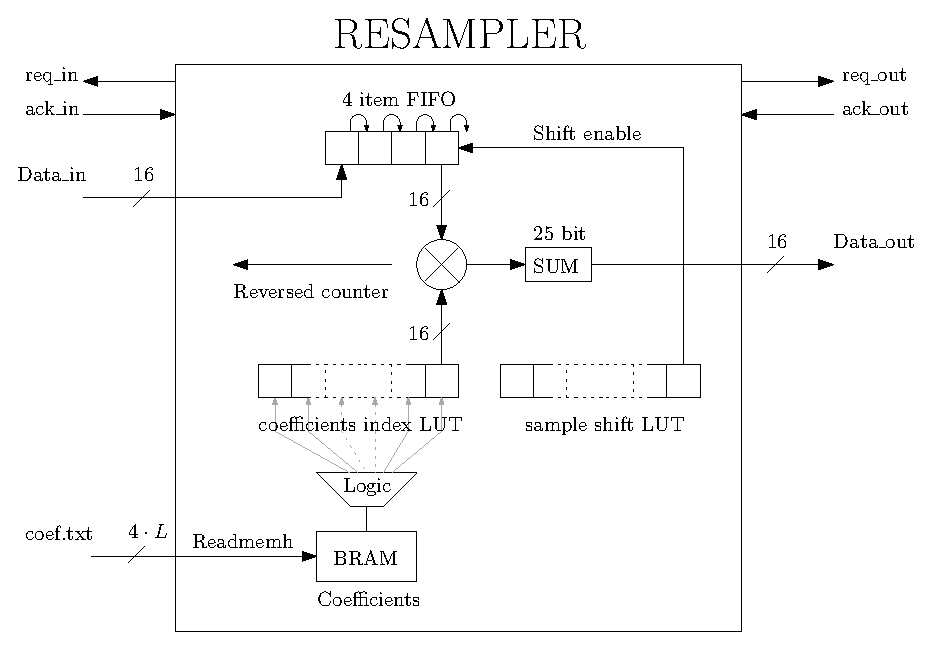
\includegraphics[scale = 1]{Images/4_blockdiagram}
    \caption{Block diagram of resampler from direct equation}
\end{figure}

\newpage
The state machine that controls the resampler is shown in the figure below:
\begin{figure}[h]
	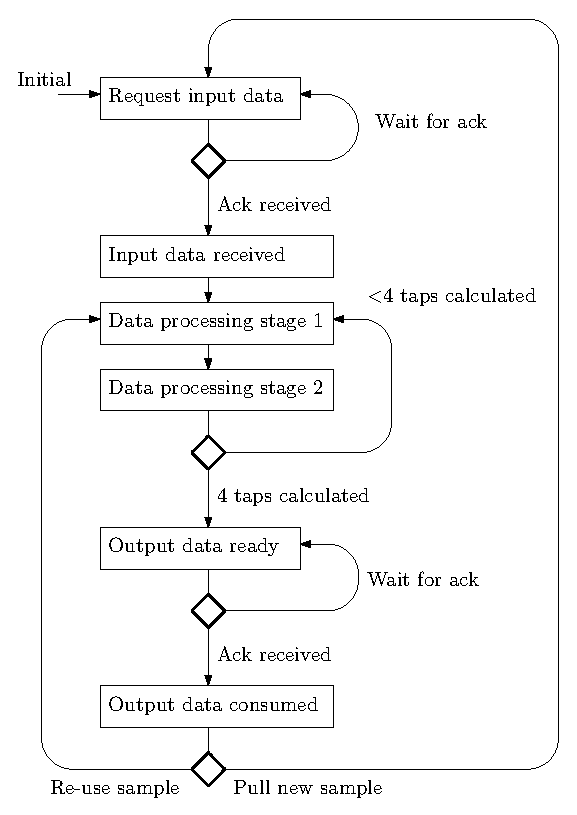
\includegraphics[scale = 1]{Images/4_statemachine}
    \caption{State machine of resampler}
\end{figure}




\newpage
\subsection{Design choices}
The resampler is based on the direct equation solution, and uses a single scaler. This is done because the naive solution needs a high internal sample frequency (that scales  with the upsample rate), and it does a lot of unnecessary multiplications by zero. It is probably possible to implemented a composite direct equation solution which shares resources (DSP units) and also uses less registers, but this will introduce additional complexity which we avoided.\\

The resampler uses a state machine that works almost identical as the standard state machine provided in lab 2 and 3. The reason why we have rewritten this state machine is that it was hard to see what was actually going on because a lot of states have almost the same requirements. Furthermore, the execution order of all states is mostly the same. Therefore, a state machine did make sense. This also allowed for easier pipelining (just split one state in two).\\

We pre-calculate the coefficients in matlab, and store them in a text-file. The matlab script is included in the appendix.\\

The coefficients are loaded in a Block RAM, and a LUT is connected to it. This LUT defines which coefficients should be used during the calculation of the current output. Another LUT is initialized to tell the system if it should re-use the current data.\\

The sum register stores the temporary results during the calculation of an output. It uses 25 bits, which are truncated to the 16 MSB when the output is ready. 
\textbf{NEED MORE ELABORATION, CANT FULLY REASON ON THIS. I THINK I ASK MONDAY}.\\

The processing step is divided in two stages: the first stage retrieves the coefficients from the BRAM with help of the coefficient LUT. The second stage computes the tap that uses this coefficients. Therefore the calculation of one output actually takes 8 clock cycles instead of 4. This choice to improve the timing constraints.

\subsection{Functional correctness}
Also see the requirements listed in section \ref{sec:req}.

\textbf{REQ 3??}

\begin{enumerate}
	\item We make use of the direct-form method, and we use set our L and M parameters to 160 and 147 respectively. This is the same ratio as $\frac{48000}{44100}$.
	\item Please see Figure~\ref{fig:compInOut} for a comparison of the input and output of the scaler.
	\item -
	\item Please see section~\ref{sec:thr4}, here we look into the timing report and note that the throughput is above 100MHz.
	\item Since we use a FIR filter, which uses samples from the past, we will have noise before our 4-sample buffer is filled.
	\item \textit{filter.v} is uses as top-level in our design.
\end{enumerate}

\subsection{Resource usage}
\label{sec:resc4}
Table~\ref{tab:4usage} summarizes the resources used by the FIR filter. This list is obtained by running the synthesis step in Xilinx ISE and extracted from the \textit{Summary} and \textit{Device Utilization} report.

\begin{table}[h]
\begin{tabular}{|l|l|l|l|}
\hline
\textbf{Resource} & \textbf{Available} & \textbf{Utilized} & \textbf{Percentage utilized}\\
\hline
Flip Flops	& 54576 & 114 	& 0 \%\\
Slice LUTs 	& 27288 & 327 	& 2 \%\\
DSP48A1s	& 58 	& 1 	& 5 \%\\
BRAM		& 116 	& 1 	& 1 \%\\
Bonded IOBs	& 218 	& 38 	& 33 \%\\
\hline
\end{tabular}
\caption{General resource usage overview}
\label{tab:4usage}
\end{table}

Only 1 DSP unit is used, this is for the multiplication in the direct form equation between the coefficient and the input.\\

Both LUTs are stored in DRAM. This is also shown in figure \ref{fig:RAM}. The shift-LUT has a size of $L\cdot 1 = 160$ bits. The coefficient index LUT requires $j\cdot DWIDTH\cdot L = 4\cdot 16 \cdot 160 = 10240$ bits of memory. This LUT is stored in 160 4x16bit RAMs, as can be seen in the figure below.\\ 

The coefficient values from the coef.txt file are stored in one Block RAM unit. One BRAM  unit of the Spartan-6 serie contains 18Kb of memory, and is therefore large enough to store all coefficient indexes. This explains the low number of used flipflops, since not many are used as a buffer.

\begin{figure}[h]
	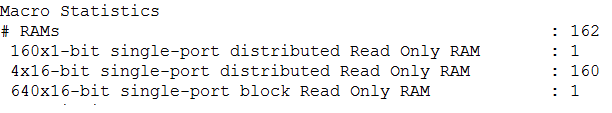
\includegraphics[scale = 0.9]{Images/simulation_missingregisters}
    \caption{Post-par RAM utilization}
    \label{fig:RAM}
\end{figure}

Furthermore, 38 IO pins are used, $16\cdot 2$ for input and output data and 6 extra for ack\_in, ack\_out, req\_in, req\_out, clk and rst.

\newpage
\subsection{System throughput and latency}
\label{sec:thr4}
The minimum sample time estimation is extracted from the \textit{Synthesis report} under \textit{Timing Report}.\\

   \textit{Minimum period:  7.464ns (Maximum Frequency: 133.981MHz)\\
   Minimum input arrival time before clock: 4.963ns\\
   Maximum output required time after clock: 3.701ns}\\

This time is equal to the largest critical path (the calculation of the tap is the critical path in this design).\\

After doing the placement and routing step, we will get a more accurate measurement of the maximum achievable throughput. These measurements can be found in the \textit{Advanced Post-PAR static timing report} under \textit{Timing summary}:\\

\textit{Minimum period:   8.164ns\{1\}   (Maximum frequency: 122.730MHz)\\
   Minimum input required time before clock:   3.971ns\\
   Maximum output delay after clock:   8.540ns}\\

Since the minimum period is the maximum delay, we can be sure that our design is able to run at 100MHz.

\newpage
\subsection{Simulation results}
See Figure~\ref{fig:compInOut} for a screenshot of Audacity comparing the input and output of the filter.

We noticed a peculiarity when comparing the input and output: the length of the output signal (in seconds) is slightly \textit{less} than the input signal. See Figure~\ref{fig:outlengdif}.

The input and output lengths are 8.454 and 8.455 seconds respectively. The output is 0.00011\% shorter. The reason of this difference in signal length is not completely clear.

\begin{figure}[h]
	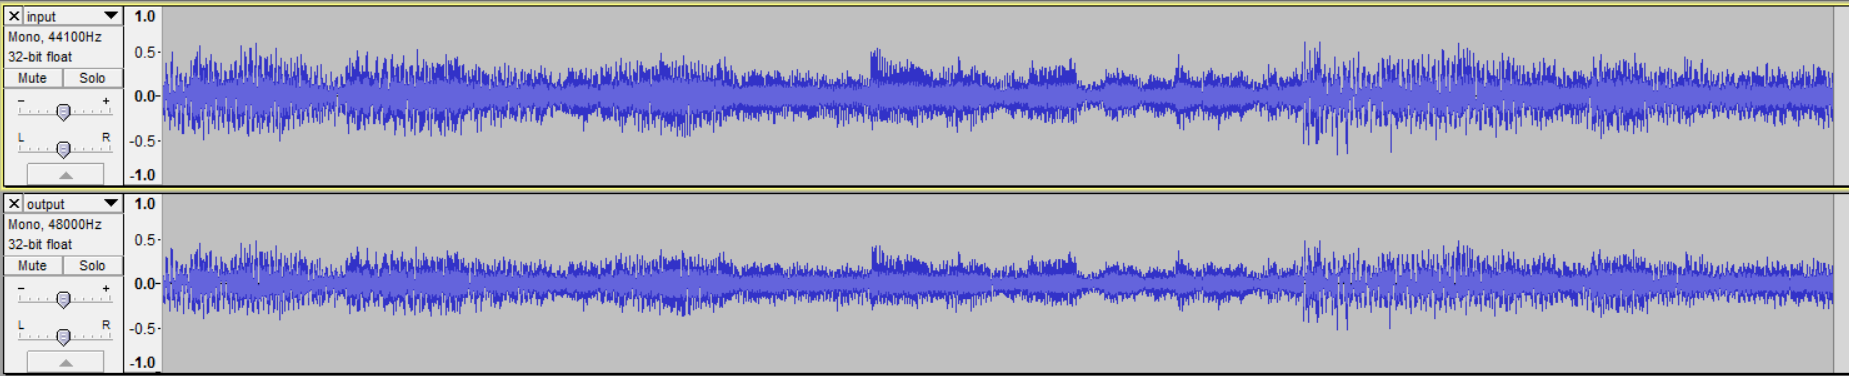
\includegraphics[scale = 0.40]{Images/simulationresults.png}
    \caption{Comparison of input and output.}
    \label{fig:compInOut}
\end{figure}

In the Audacity frequency plot we saw a few noteworthy difference. At first, the output spectrum is a bit weaker overall. This is probably due to rounding. The second thing is that after 18khz, the output signal has some additional noise. 

\begin{figure}[h]
	\begin{subfigure}[b]{0.45\textwidth}	
		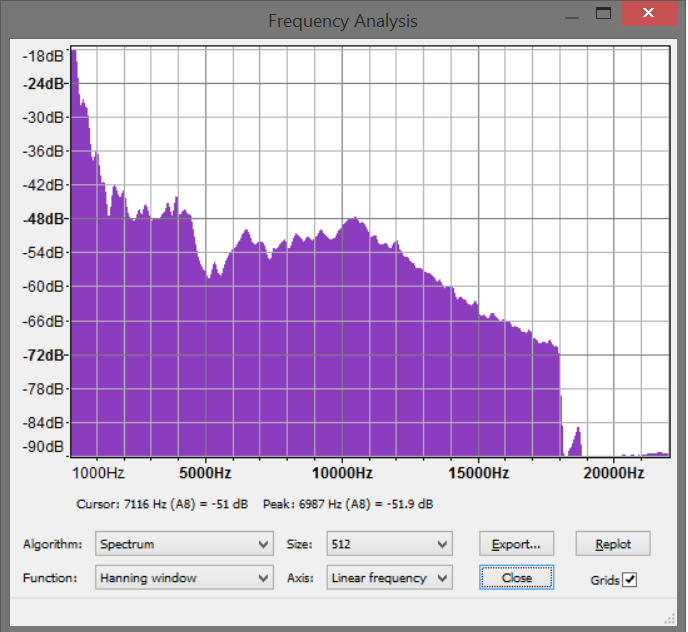
\includegraphics[scale=0.5]{Images/simulation_frequencyspectrum_input.png}
	\end{subfigure}
	\begin{subfigure}[b]{0.45\textwidth}	
		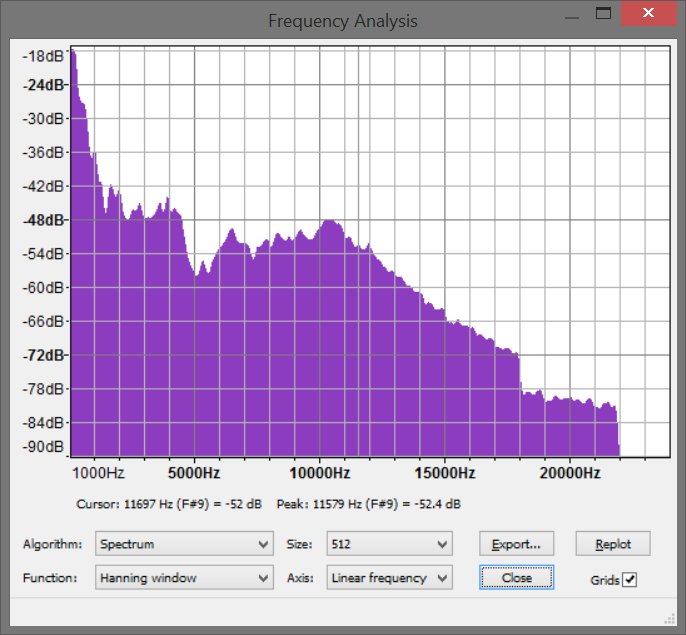
\includegraphics[scale=0.5]{Images/simulation_frequencyspectrum_output.png}
	\end{subfigure}
    \caption{Comparison of the input spectrum (left) and output spectrum (right).}
\end{figure}
\clearpage


\section{Appendix A: Matlab coefficients script}
\begin{lstlisting}
% Put this in a file named coef_generate_matlab.m, then call it 
% while you are in the file directory. It will write the coefficients
% to the coef.txt file and also return them.

function [y] = coef_generate_matlab(L)
        % make sure that coefficients sum to 1
        y = coef_gen(L);
        y = y/sum(y);

        % quantize and round to nearest integer
        y = round(y*(2^16)); 
             
        % convert to signed int filter coeff
        y = int16(y);
        y = hex(fi(y, 1, 16, 0)); %1 stands for signed, 16 bit out
        
        dlmwrite('coef.txt',y,''); %create file, with no delimiter ''      
end

function [y] = coef_gen(L)
    % generate 4*L coefficients and start at 0 instead of 1 *stupid matlab*
    for n = 1:4*L
            y(n) = lanczos2(((n-1)/L) -2);
    end
end

function y = lanczos2(t)
    if(t <= -2 || t >= 2)
        y = 0;
    else
        y = sinc(t).*sinc(t/2);
    end
end
\end{lstlisting}

Figure~\ref{fig:frq} shows the frequency response of the FIR filter that is generated with help of the matlab code from appendix A.

\begin{figure}[h]
	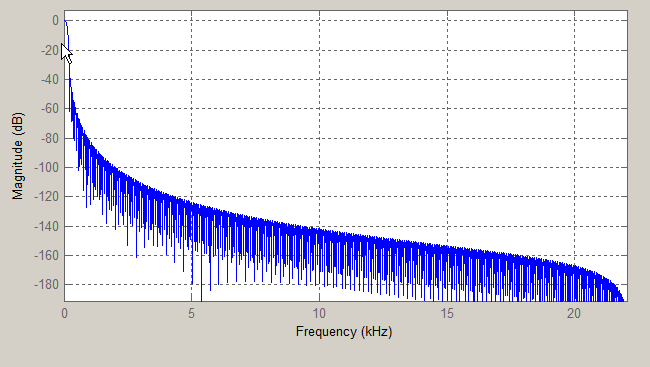
\includegraphics[scale=0.7]{Images/frequencyplot}
    \caption{Interpolation filter frequency domain (Matlab)}
    \label{fig:frq}
\end{figure}

\newpage
\section{Appendix B: Verilog Code}
File: filter.v.
\begin{lstlisting}[language=Verilog]
`timescale 1ns / 1ps

module filter
       #(parameter DWIDTH = 16,
         parameter DDWIDTH = 2*DWIDTH,
         parameter L = 160,
         parameter L_LOG = 8,
         parameter M = 147,
         parameter M_LOG = 8,
         parameter CWIDTH = 4*L)
       (input clk,
        input rst,
        output req_in,
        input ack_in,
        input signed [0:DWIDTH-1] data_in,
        output req_out,
        input ack_out,
        output signed [0:DWIDTH-1] data_out);

// Output request register
reg req_out_buf;
assign req_out = req_out_buf;

// Input request register
reg req_in_buf;
assign req_in = req_in_buf;

// Accumulator and temporary buffer
reg signed [0:DDWIDTH-8] sum; //25 bit!
reg signed [0:DWIDTH-1] data_out_buf;
assign data_out = data_out_buf;

//coefficients data and lookup tables for the coef index and shift index
reg signed [0:DWIDTH-1] mem[0:3],
    coef_buf,
    coef [0:CWIDTH-1], //** means 'power'
    lookup_coefIdx[0:L-1][0:3];
reg [0:L-1]lookup_shift; //'1' means shift, '0' means no shift

integer i, j, cnt;
initial begin
    // import coefficients
    $readmemh("coef.txt", coef, 0, CWIDTH -1);

    // define lookup tables
    for (i = 0; i < L; i = i + 1) begin
        for (j = 0; j < 4; j = j +1) begin
            lookup_coefIdx[i][j] = j*L + i*M%L;
        end

        if(i*M/L == (i+1)*M/L)
            lookup_shift[i] = 0; //do not shift yet
        else
            lookup_shift[i] = 1; //shift
    end
end

// State machine variables
reg [3:0] state;
parameter input_data_requested 	= 1,
          input_data_received 	= 2,
          output_data_consumed 	= 3,
          output_data_ready 		= 4,
          data_processing_stage1 = 5,
          data_processing_stage2 = 6,
          waiting_for_ack 			= 7;

// State machine that controls the flow control between testbench and filter
always @(posedge clk) begin
    if (rst) begin
        req_in_buf <= 0;
        req_out_buf <= 0;
        sum <= 0;
        cnt <= 3;
        i <= 0;
        state <= 0;
    end
    else begin
        case (state)
            waiting_for_ack: begin
                if(req_in && ack_in)
                    state <= input_data_received;

                if (req_out && ack_out)
                    state <= output_data_consumed;
            end

            input_data_requested: begin
                req_in_buf <= 1;
                state <= waiting_for_ack;
            end

            input_data_received: begin
                mem[0] <= data_in;

                req_in_buf <= 0;
                state <= data_processing_stage1;
            end

            // stage 1 of data processing to get the coefficients **pipelining**
            data_processing_stage1: begin
                // get coefficient for next run **reduce pipeline**
                coef_buf <= coef[lookup_coefIdx[i][cnt]];

                state <= data_processing_stage2;
            end

            // stage 2 of data processing to calculate one of the 4 taps
            data_processing_stage2: begin
                // shift the data, but only if we do not have to re-use it once more after this
                mem[cnt+lookup_shift[i]] <= mem[cnt];
                sum <= sum + mem[cnt]*coef_buf;

                cnt <= cnt - 1;

                if(cnt == 0)
                    state <= output_data_ready;
                else
                    state <= data_processing_stage1;
            end

            output_data_ready: begin
                data_out_buf <= sum[0:15];
                cnt <= 3;

                req_out_buf <= 1;
                state <= waiting_for_ack;
            end

            output_data_consumed: begin
                // reset variables and increment index
                sum <= 0;
                i <= (i + 1) % L;

                req_out_buf <= 0;
                if (lookup_shift[i] == 1)
                    state <= input_data_requested;
                else
                    state <= data_processing_stage1; 
            end

            default: begin
                state <= input_data_requested;
            end
        endcase
    end
end
endmodule
\end{lstlisting}

\end{document}
